\documentclass{article}

\usepackage{amsmath}
\usepackage{amsfonts}
\usepackage{url}
\usepackage[utf8]{inputenc}
\usepackage{graphicx}
\usepackage{multicol}

\setlength{\parskip}{1em}

\graphicspath{ {./images_dataset/} }

\begin{document}
% ==============================================================
\section{Generative Adversarial Networks}


Introduced in 2014 \cite{goodfellow_generative_2014}, generative adversarial  networks, so-called GANs, have been the focus of countless research papers and creative implementations.

We can train them to generate new samples from a given distribution without the difficulties of approximating likelihood functions. In order to do so, we train two neural networks to compete with each other. The discriminator network is trained to tell apart real samples from "fake" samples, while the generator network tries to generate samples that will fool the discriminator.

% ==============================================================
\subsection{Training Objective}
Given input data with distribution $p(x)$, the generator $G$ is a neural network, that maps random input noise $z$ to the input space, as $G(z, \theta_{g})$, learning the model distribution $\hat{p}(x)$. The discriminator $D$ is a second neural network $D(x, \theta_{d})$ with a single scalar output, classifying the input as real, sampled from $p(x)$, or as fake, sampled from the model distribution $\hat{p}(x)$. 

The training objective of the discriminator is to maximize the probability of assigning the correct label, while the objective of the generator is to minimize this probability. The loss function of the GAN can be described as the minimax objective,

\begin{equation}
\underset{G}{\mathrm{min}} \ \underset{D}{\mathrm{max}} \ V(D,G) = \mathbb{E}_{x \sim p_{data}(x)}[\log D(x)] + \mathbb{E}_{z \sim p_{z}(z)}[\log 1 - D(G(z))]
\label{eq:minimax}
\end{equation}.

In order to prevent vanish gradients, as a result of the discriminator saturating by confidently classifying the samples before the generator's update, \cite{goodfellow_generative_2014} suggests $G$ to be trained to maximize $\mathbb{E}_{z \sim p_{z}(z)}[\log D(G(z))]$ instead.

% ==============================================================
\subsection{Training Difficulties}
In theory, the minimax game described in equation \ref{eq:minimax} is played until generator has perfectly modeled the distribution $p(x)$, so that discriminator classifies the authenticity of the samples at random. 

In reality, finding the right balance between the two networks is one of the difficulties when training a GAN. If discriminator gets too good at determining which samples are fake, then generator has no chance to learn the distribution. On the other hand, if generator is updated too much, it can collapse too many values of $z$ to the same value of $x$ to have enough diversity to model the distribution.

% ==============================================================
\section{GAN Comparison}
Lot of papers and open-source repositories have been published since the appearance of the original GAN paper. I have reviewed and tested several of them, in order to find architectures and code applicable to the problem of generating and modifying fashion images. 

\begin{table}
\centering
\begin{tabular}{l*{4}{c}}
Network Characteristics & pix2pix &	StarGAN	& MUNIT	& FaderNetworks \\
\hline
Supervised Training		& Yes & No & No & No \\
Multi-Domain  			& No  & Yes & No & No \\
Multi-Modal				& No & No & Yes & No \\
Latent Representations	& No & No & Yes & Yes \\
\end{tabular}
\caption{\label{tab:gan_comp}\textbf{Comparison of existing GAN models based on their characteristics.} Supervised training means that the dataset consists of image pairs, e.g: a dress and a person wearing the dress. Multi-Domain networks are able to train one model to change multiple attributes. Multi-Modal networks are able to generate more than one possible output. Networks with latent representations try to model the training data in a latent space, as opposed to pixel space.}
\end{table}

Based on various characteristics, compared in Table \ref{tab:gan_comp}, I have evaluated  5 networks: pix2pix \cite{isola_image--image_2016}, CycleGAN \cite{zhu_unpaired_2017}, StarGAN \cite{choi_stargan:_2017}, MUNIT \cite{huang_multimodal_2018} and FaderNetworks \cite{lample_fader_2017}. I have compared the following attributes for each of the mentioned networks:
\begin{itemize}
\item Supervised/Unsupervised learning: Describes if the network needs a dataset consisting of paired images, such as the same skirt in a short and log version.
\item Multi-Domain: Describes if the network is able to train only one model for different domain modifications, or if each domain requieres its own trained generator.
\item Multi-Modal: Describes if the network is able to generate different versions from the same input.
\item Latent representation: Describes if the network trains directly in pixel-space or uses latent representation of the data, usually content and style of the images.
\end{itemize}

% ==============================================================
\subsection{Pix2Pix}
The so-called pix2pix networks were first introduced by Isola et al. \cite{isola_image--image_2016} as a framework for image-to-image translations using conditional neural networks. Some of the applications of pix2pix include mapping day photographs to night, sketches of shoes to realistic shoe images or colorizing black-and-white photos.

Pix2Pix uses the concept of conditional GANs \cite{mirza_conditional_2014}, where the network's output can be influenced by providing a class label $c$. The class label is fed to both the generator $G(z|c)$ and discriminator $D(x|c)$ as an additional input layer.

In case of pix2pix, the network is trained to translate images from an input domain to a target domain, requiring a dataset of paired images $(x_{input}, x_{target})$, such as a photograph of a street during the day and a corresponding night photograph of the same street. In addition to the generator mapping the random noise $z$ to target domain $\hat{x}_{target}$, it is also conditioned on the input image $x_{input}$, such as $G: (x_{input}, z) \rightarrow \hat{x}_{target}$.

The adversarial objective, which $G$ is trained to minimize and $D$ is trained to maximize, can be expressed as following:

\begin{equation}
\mathcal{L}_{adv}(D,G) = \mathbb{E}_{x_{in},x_{trg}}[\log D(x_{in},x_{trg})] + \mathbb{E}_{x_{in},z}[\log 1 - D(x_{in}, G(x_{in},z))]
\label{eq:pix2pix_minimax_cond}
\end{equation}

Based on the results of previous conditional GAN approaches \cite{pathak_context_2016}, Isola et. al \cite{isola_image--image_2016} have also shown, that enforcing the generated output to be closer to the ground truth target by adding a second objective reduces artifacts in the results. They therefore suggest to use the L1 distance as reconstruction loss function for the generator to optimize.

\begin{equation}
\mathcal{L}_{rec}(G) = \mathbb{E}_{x_{in},x_{trg},z}[||x_{trg}-G(x_{in},z)||_{1}]
\label{eq:pix2pix_loss_rec}
\end{equation}


The final objective of the generator is:
\begin{equation}
G^{*} = arg \ \underset{G}{\mathrm{min}} \ \underset{D}{\mathrm{max}} \ \mathcal{L}_{adv}(D,G) + \lambda \mathcal{L}_{rec}(G)
\end{equation}
with the optimal $\lambda$ = 100.


% ==============================================================
\section{Fashion Dataset}
As in most machine learning algorithms applied to visual tasks, the quantity and quality of training data is essential to produce high-quality results. It is also common, that data collection and data cleaning make up a significant part of a machine learning project.

In case of fashion images, there are several open-source datasets published online, however, after careful evaluation I have not found them sufficient for the type of tasks I wanted to achieve. Therefore, I have created an application that can scrape an online fashion store to download images of fashion products and their description to an easily-accessible format.

% ==============================================================
\subsection {Requirements}
In order to generate high-quality outputs using GANs, the collected dataset should fulfill the following requirements as much as possible:
\begin{enumerate}
\item The fashion products should be photographed on a white background.
\item There should be a machine-readable description of each product, such as color, shape, category, etc.
\item The images should be in a sufficient resolution.
\item There should be a sufficient amount of images of various items.

\end{enumerate}
I have defined these requirements on based on my previous experience with generative algorithms. 

% ==============================================================
\subsection {Existing Fashion Datasets}

\subsubsection{DeepFashion}
The existing datasets that consist or include images of fashion items do not fulfill the criteria of the dataset for the application. The Deep Fashion Set includes a very extensive Attribute Prediction collection, with more than 200.000 images of clothing images, labeled with 1000 attributes \cite{the_chinese_university_of_hong_kong_deepfashion_nodate}. However, this dataset does not fulfill the first requirement, with its clothing items photographed on people in various poses and backgrounds. This type of variation might be too complex for the algorithms and can lead to unsatisfactory results.

\subsubsection{Pixabay and Fotolia}
Another available option, that has been provided by Prof. Dr. Barthel, was the Fotolia and Pixabay image datasets, which can be explored on the picsbuffet website \cite{noauthor_picsbuffet_nodate}.

Based on 64-dimensional feature vectors calculated via the akiwi API, figure 1 shows images with the closest L1 distance to the template image and keywords "dress" and "isolated". 

\begin{figure}[h]
\begin{multicols}{3}
\centering
\fbox{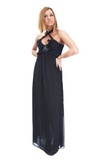
\includegraphics[width=.3\textwidth]{fotolia_ex1}}\hfill
\fbox{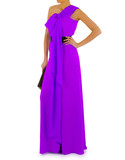
\includegraphics[width=.3\textwidth]{fotolia_ex2}}\hfill
\fbox{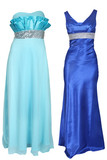
\includegraphics[width=.3\textwidth]{fotolia_ex3}}\hfill
\end{multicols}
\caption{Example of a parametric plot ($\sin (x), \cos(x), x$)}
\end{figure}


However, in addition to the problem with too much variety as in DeepFashion, the attributes saved for each item did not prove to be useful and the images did not have sufficient resolution. 




\bibliographystyle{alphadin}
\bibliography{Zotero}
\end{document}
